\subsection{Trực quan hóa: Số chiều – 2 chiều (2D)}
\textit{VisuExplore} [338] là một hệ thống tương tác trực quan phục vụ cho việc khai phá chuỗi các dữ liệu, thông số y tế không đồng nhất theo thời gian. Hệ thống này sử dụng nhiều chế độ xem khác nhau nằm song song với nhau theo chiều dọc với chung một trục hoành là trục thời gian, từ đó giúp cho việc tham chiếu các thông số y tế có liên quan với nhau. VisuExplore cung cấp một môi trường mở rộng chứa các công cụ, kỹ thuật hiển thị trực quan với tôn chỉ đơn giản, dễ dàng sử dụng trong thực hành y tế như: biểu đồ đường, biểu đồ dòng thời gian (timeline), biểu đồ cột, biểu đồ miền [331], biểu đồ sự kiện, biểu đồ đường với chú thích có thể thu phóng (xem Hình (\ref{fig:f7.14}), trên cùng). Ngoài ra, dữ liệu cũng có thể được trình bày dưới dạng các bảng chứa văn bản để đa dạng các cách thức trực quan hóa. Các tính năng tương tác của VisuExplore cho phép các bác sĩ có được cái nhìn tổng quan về nhiều thông số y tế và tập trung vào các phần của dữ liệu. Có thể thêm hình ảnh hiển thị một hoặc nhiều biến bổ sung. Người dùng có thể thêm, xóa, thay đổi kích thước và sắp xếp lại các chế độ xem trực quan hóa vì VisuExplore cũng cung cấp khả năng tương tác phong phú để thêm, xóa, sắp xếp và điều chỉnh chế độ xem. Ngoài ra, một công cụ đo lường cũng được tích hợp để có thể xác định khoảng thời gian giữa các hai thời điểm mà người dùng quan tâm và lựa chọn; chức năng này không hoạt động trong phạm vi của một chế độ xem cụ thể mà còn có thể hoạt động xuyên suốt trên các chế độ xem khác nhau.
\begin{figure}[H] % places figure environment here   
    \centering % Centers Graphic
    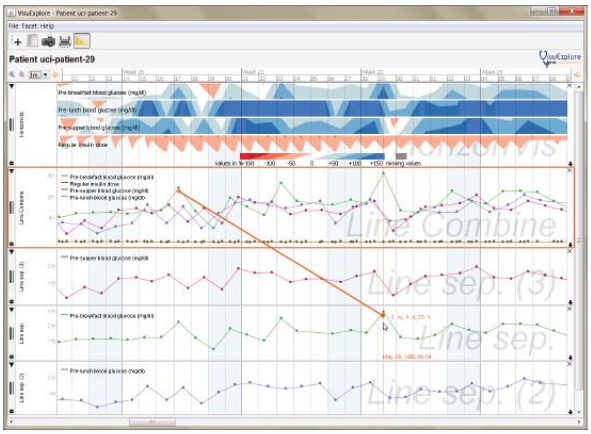
\includegraphics[width=0.8\textwidth]{assets/fig_7_14.png} 
    \caption{VisuExplore [338]. Các phương pháp biểu diễn trực quan, đơn giản và dễ hiểu bằng cách sử dụng biểu đồ đường, biểu đồ cột, biểu đồ sự kiện, biểu đồ dòng thời gian và biểu đồ đường kèm chú thích. Trong đó, công cụ đo lường được minh họa: Một đường nối minh họa cho khoảng thời gian giữa hai mục được chọn (đường nối này hoạt động trên các khung khác nhau). (Được tạo bằng phần mềm nguyên mẫu VisuExplore.)} % Creates caption underneath graph
    \label{fig:f7.14}
\end{figure}